\chapter{Background and Motivation} \label{chap:chap-1}

\section{Image-guided Percutaneous Interventions}
\label{sec:image-guided-percutanous-interventions}

Percutaneous needle interventions \added[id=ii]{are medical procedures where a thin needles is inserted through the skin to access various organs or tissues for diagnostic or therapeutic purposes. These image-guided interventions} capture a broad class of minimally invasive diagnosis and treatment procedures, such as biopsy~\parencite{bourgouinImageGuidedPercutaneousLung2021, birginCoreNeedleBiopsy2020, shethSocietyInterventionalRadiology2020, wuComplicationsCTGuidedPercutaneous2011}, brachytherapy~\parencite{chargariBrachytherapyOverviewClinicians2019, ragdeModernProstateBrachytherapy2000, wanBrachytherapyNeedleDeflection2005, podderVivoMotionForce2006}, and spinal injection~\parencite{wonFacetJointInjections2020,manchikantiEpiduralInterventionsManagement2021, carassitiEpiduralSteroidInjections2021, silbergleitImagingguidedInjectionTechniques2001}.

\added[id=ak]{For example, transthoracic needle biopsy (TTNB) is a procedure used to obtain tissue samples from the lung for diagnostic evaluation, and is typically performed under imaging guidance (e.g. CT) using a fine needle (fine-needle aspiration, FNA) or a core needle (core biopsy)~\mbox{\parencite{dibardinoTransthoracicNeedleBiopsy,tsukadaDiagnosticAccuracyCTGuided2000,tomiyamaCTguidedNeedleBiopsy2006}}. Medical conditions that can be identified by TTNB include primary lung cancer~\mbox{\parencite{myersLungAdenocarcinoma2025,demargerie-mellonImageguidedBiopsyPrimary2016}}, pulmonary tuberculosis~\mbox{\parencite{lyonPulmonaryTuberculosis2017,cicenasLungCancerPatients2007}}, and hamartomas~\mbox{\parencite{gjevrePulmonaryHamartomas1996}}. Reports have shown that lesion size is a determining factor in diagnostic accuracy, with smaller lesions leading to less accurate diagnosis: for lesions 31-50 mm in diameter, the diagnostic accuracy is 93.3\%, but drops to 66.7\% when the lesion diameter decreases to 6-10 mm~\parencite{tsukadaDiagnosticAccuracyCTGuided2000}. Air embolism can also occur during rapid inspiration when the tip of biopsy needle is lodged in pulmonary vein and inner stylet is removed, thus making a precise needle insertion paramount in diagnosis accuracy~\parencite{wuComplicationsCTGuidedPercutaneous2011}.}

\added[id=ak]{Another needle-based percutaneous procedure is spinal injection, which is used to diagnose and treat pain originating from the spine. These procedures typically involve injecting medications such as corticosteroids, local anesthetics, or anti-inflammatory drugs near spinal nerves, joints, or the epidural space to relieve pain and inflammation~\mbox{\parencite{wonFacetJointInjections2020,silbergleitImagingguidedInjectionTechniques2001, manchikantiEpiduralInterventionsManagement2021,carassitiEpiduralSteroidInjections2021}}. Serious complications, such as sciatic nerve injury during intramuscular injections, can lead to complete paralysis if the injection is misplaced or administered with poor technique~\parencite{jungkimSciaticNerveInjection2014,parkIatrogenicInjurySciatic2019}. Spinal anesthesia can also develop when the needle goes past the intended target and into the spinal cord~\parencite{bogdukComplicationsSpinalDiagnostic2008}.}

\added[id=ii]{For example,~\cref{fig:chap-2-percutaneous-intervention} shows an example CT-guided lung needle biopsy and a fluoroscopy-guided diagnostic injection of a lumbar facet joint.}

\begin{figure}[h]
  \centering
  \includegraphics[width=0.68\columnwidth]{figures/medical_images/percutaneous_intervention.png}
  \caption{Examples of image-guided percutaneous interventions: (a) CT-guided lung needle biopsy and (b) fluoroscopy-guided diagnostic injection of a lumbar facet joint. Image credit~\parencite{bourgouinImageGuidedPercutaneousLung2021, fritzManagementChronicLow2007}.}
  \label{fig:chap-2-percutaneous-intervention}
\end{figure}

Depending on the clinical procedure, a wide range of needles with different gauges, stiffness, and tip geometries are available. These inherent needle characteristics play a crucial role in determining how the needle moves through biological soft tissues; additionally, surgeons also employ various freehand techniques, such as rotating or bending the needle, to adjust the needle tip position \textit{in situ} during insertion~\parencite{calthorpeHistorySpinalNeedles2004,tsenNeedlesUsedSpinal2006,fritzAugmentedRealityVisualization2012,bourgouinImageGuidedPercutaneousLung2021,kimConsiderationsFluoroscopicGuided2020,shanahanComparisonPermanentProstate2002}. \added[id=ak]{For example,~\parencite{bourgouinImageGuidedPercutaneousLung2021} reports a ``banana bend'' technique to adjust needle trajectories during lung biopsy (see~\cref{fig:chap-1-banana-bend}),~\parencite{kimConsiderationsFluoroscopicGuided2020} reports a ``leverage'' method for adjusting a partially inserted needle during fluoroscopy-guided spinal blocks, and~\parencite{shanahanComparisonPermanentProstate2002,bernardesDataDrivenAdaptiveNeedle2023} report the use of a ``Diddler'' to adjust the position of transperineal needles during prostate brachytherapy.}

\begin{figure}[ht]
  \centering
  \includegraphics[width=0.68\columnwidth]{./figures/medical_images/banana-bend.jpg}
  \caption{A ``banana bend'' technique for adjusting needle trajectory during CT-guided lung needle biopsy. Image credit~\parencite{bourgouinImageGuidedPercutaneousLung2021}.}
  \label{fig:chap-1-banana-bend}
\end{figure}

Despite the prevalent use of intraoperative medical imaging as a way of visual feedback to the clinicians, successful placement of the flexible needle using freehand techniques is still challenging. As an example, for a standard ultrasound-guided 12-core prostate biopsy, false negative rate still exceeds 30\% -- a problem that persists even with repeated interventions~\parencite{serefogluHowReliable12Core2013}. This issue is compounded by inherent undersampling, which emphasizes the need for precise placement of the biopsy needle to effectively mitigate diagnostic challenges~\parencite{prestiProstateBiopsyCurrent2007}.

\deleted[id=ak]{Additionally, complications due to imprecise needle insertion can be damaging and even life threatening. For example, during CT-guided percutaneous needle biopsy of the chest, if the tip of biopsy needle is lodged in pulmonary vein and inner stylet is removed, air embolism can occur during rapid inspiration when atmospheric pressure exceeds pulmonary venous pressure~\parencite{wuComplicationsCTGuidedPercutaneous2011}. During fluoroscopy-guided intra-articular spinal injection procedures, the needle can go past the intended target and into the spinal cord, resulting in high spinal anesthesia~\parencite{bogdukComplicationsSpinalDiagnostic2008}.}

In general, image-guided percutaneous needle interventions are minimally invasive, but patient outcomes correlate directly to the accuracy of needle placement. Here, we highlight the following challenges regarding freehand needle insertions under imaging guidance:
\begin{enumerate}
\item Frequency of image acquisition and exposure to ionizing radiation.
\item Accuracy of image interpretation and mental correlation with needle in hand.
\item Experience-based freehand maneuvers informed by imaging and haptic feedback from needle.
\end{enumerate}

The following section illustrates how modern medical robotics, particularly those using magnetic resonance imaging (MRI), can help address \replaced[id=ak]{challenges 1 and 2}{some of these challenges}.

\section{\replaced[id=ak]{MRI}{Image}-guided Needle Positioning Robots}
\label{sec:image-guided-needle-positioning-robots}

MRI offers a unique set of advantages over other imaging modalities for image-guided interventions, such as superior soft tissue contrast, real-time capability, and free of ionizing radiation~\parencite{tsekosMagneticResonanceCompatible2007}. However, one critical limitation for the MRI-guided approach is the difficulty to access the patient anatomy of interest due to the limited space in the scanner bore; thus, remotely actuated and controlled robots have been introduced to take advantage of this imaging modality. Susil et al. developed an MR-compatible transrectal system to perform MRI-guided prostate biopsy procedures~\parencite{susilSystemMRImage2003, susilSystemProstateBrachytherapy2004}, and the device was further improved by Krieger et al.~\parencite{kriegerDesignNovelMRI2005}. This remotely actuated manipulator was able to place the needle tip to less than 2.3 mm from the target. Fischer et al. developed a pneumatically actuated needle placement device for real-time MRI-guided  transperineal prostate interventions~\parencite{fischerMRICompatiblePneumaticRobot2008}. Patel et al. designed a patient-mounted, 4 degree-of-freedom (DOF) robot actuated by piezoelectric motors for MRI-guided shoulder arthrography~\parencite{patelRoboticSystemMRIGuided2018}. Wu et al. designed a remotely actuated needle driving device that allows clinician to manually steer and insert the needle away from the scanner bore~\parencite{wuRemotelyActuatedNeedle2019}, and is incorporated into a 6-DOF robot for MRI-guided low back pain injection procedures~\parencite{liFullyActuatedBodyMounted2020a}. Stoianovici et al. developed an MR-Safe robotic system that employs a parallelogram-type mechanism to physically enforce an RCM below the needle guide, and was able to achieve high structural stiffness and targeting accuracy~\parencite{stoianoviciMultiImagerCompatibleMR2018}. 

Most of the above systems focus on the design, material selection, and MRI-compatibility, and integrated workflow of robot-assisted needle insertions. These robots have high accuracy in free space -- they are able to move the needle precisely to the entry point based on pre-operative imaging, yet, as highlighted in~\parencite{moreiraEvaluationRobotAssistedMRIGuided2018}, ``needle deviation $\cdots$ was primarily influenced by the interaction between the needle and the skin, which was represented by the deviation at the entry point'', and ``(t)he elastic contact during the puncture deviated the needle from the intended path at the beginning of the needle path''. In other words, high precision in robot motion and image registration is only a necessary condition for accurate needle insertions; \emph{feedback and control algorithms informed by physical understanding of the surgical scenario is equally important}.

\section{Steering of Hyper-flexible Bevel-tip Needles}
\label{sec:steering-of-hyperflexible-bevel-tip-needles}

A plethora of needle insertion research falls under \textit{steering} of bevel-tip needles, where it is assumed that the needle follows its tip exactly and steering is achieved only via axial rotation~\parencite{liReviewTechniquesUsed2022}. These \textit{steering} models are largely derived from vehicle kinematics, where nonholonomic motion constraints restrict control inputs to insertion and bevel rotation; however, these models assume that needle flexibility is negligible compared to surrounding tissues -- an assumption rarely practical in clinical settings due to the inherent stiffness of off-the-shelf medical needles.

In order to create a working environment for these nonholonomic models, the ``needles'' are often replaced by thin nitinol wires that have low bending stiffness that allows their trajectory to be defined primarily by the tip of the instrument. Decreased bending stiffness also leads to needle buckling upon contact with human skin, making it challenging to penetrate the protective layer of muscle tissues. Further, the mode of needle control is restricted to axial rotation and insertion, since any other manipulation of the needle results immediately to large needle deformation and violates the kinematic constraints of the model.

% \subsection{Nonholonomic Bicycle Model for Bevel-tip Needles}
% \label{sec:bevel-tip-model}

% Here we present the full derivation of the kinematics of a bicycle model. The fixed-steer bicycle is a common model for the tip of a beveled needle, and is very commonly used in trajectory planning for needle insertion.

% To have better model compatibility with conventions used in continuum mechanics (beam and rod, to be specific), we use the following convention: insertion/longitudinal axis is $x$, bevel/bending axis is $y$, and their binormal is $z$. Using a right-handed Cartesian coordinate, $x$ is positive to the right, $y$ positive upward, and $z$ positive out-of-page. 

% We establish an inertial frame $\lbrace W\rbrace$, then a bicycle model has two frames: a rear wheel/base frame $\lbrace B\rbrace$and a front wheel/tip frame $\lbrace T\rbrace$ located $l$ distance apart in the $x$-direction of $\lbrace B\rbrace$. To create a bevel/bending effect along insertion, we rotate $\lbrace T\rbrace$ along local $z$-axis by $\varphi$, therefore the homogeneous transformation from $\lbrace B\rbrace$ to $\lbrace T\rbrace$ is $g_{bt} =\left(R_z (\phi ),[l,0,0]^{\top } \right)$, i.e.
% \begin{equation}
%   \label{eq:chap-1-gbt}
%   g_{bt} =
%   \begin{bmatrix}
%     \cos{\phi} & -\sin{\phi} & 0 & l \\
%     \sin{\phi} & \cos{\phi} & 0 & 0 \\
%     0 & 0 & 1 & 0 \\
%     0 & 0 & 0 & 1
%   \end{bmatrix}
% \end{equation}

% The kinematic chain from the inertial frame to the the tip frame is $g_{wt} =g_{wb} g_{bt}$, and the body velocity is therefore
% \begin{equation}
%   \label{eq:chap-1-body-vel}
%  {\hat{\zeta} }_{wt} =g_{wt}^{-1} \dot{g_{wt} } ={\left(g_{wb} g_{bt} \right)}^{-1} \dot{\left(g_{wb} g_{bt} \right)} =g_{bt}^{-1} \left(g_{wb}^{-1} \dot{g_{wb} } \right)g_{bt}
% \end{equation}

% We use the $\ad$ operator to rewrite the above equation in vector format:
% \begin{equation}
%   \zeta_{wt} = \ad_{g_{bt}^{-1}}\zeta_{wb} =
%   \begin{bmatrix}
%     v_1\cos{\phi} +v_2\sin{\phi}+lw_3\sin{\phi}\\
%     v_2\cos{\phi} -v_1\sin{\phi}+lw_3\cos{\phi}\\
%     v_3 -lw_2 \\
%     w_1\cos{\phi}+w_2\sin{\phi}\\
%     w_2\cos{\phi}-w_1\sin{\phi}\\
%     w_3 
%   \end{bmatrix}
% \end{equation}

% In local frames, nonholonomic motion constraints requries $\zeta_{wb} (2)=\zeta_{wb} (3)=\zeta_{bt} (2)=\zeta_{bt} (3)=0$, in other words, there cannot be instantaneous lateral movement for frames $\lbrace B\rbrace$ and $\lbrace T\rbrace$. This can be expressed in a Pfaffian constraint format as
% \begin{equation}
%   0=A\dot{q} \quad \text{where} \quad
%   A=
%   \begin{bmatrix}
%     0 & 1 & 0 & 0 & 0 & 0\\
%     0 & 0 & 1 & 0 & 0 & 0\\
%     0 & 0 & 0 & 0 & 1 & 0\\
%     -\frac{\tan \left(\varphi \right)}{l} & 0 & 0 & 0 & 0 & 1
%   \end{bmatrix}\quad \text{and} \quad
%   \dot{q} =
%   \begin{bmatrix} v_1 \\ v_2 \\ v_3 \\ w_1 \\ w_2 \\ w_3     
%   \end{bmatrix}
% \end{equation}

% Noticing that the two hyperparameters can be groupled into one term $\kappa = -\frac{\tan{\phi}}{l}$, the allowable velocities are contained in 
% \begin{equation}
%   U = \mnull{(A)} =
%   \begin{bmatrix}
%     0 & -\frac{1}{\kappa }\\
%     0 & 0\\
%     0 & 0\\
%     1 & 0\\
%     0 & 0\\
%     0 & 1
%   \end{bmatrix}
% \end{equation}
% Thus, letting $\zeta_1 =U\left(:,1\right)$ and $\zeta_2 =U\left(:,2\right)$, we have $\zeta_{wt} =\zeta_1 u_1 +\zeta_2 u_2 ={\left(g_{wt}^{-1} \dot{g_{wt} } \right)}^{\vee }$.

% We parameterize $g_{wt} =\left(R_{wt} ,p_{wt} \right)$ by states ${\left\lbrack x,y,z,\alpha ,\beta \;,\gamma \right\rbrack }^{\top }$, such that $R_{wt} =Rot_i (\alpha )Rot_j (\beta )Rot_k (\gamma )$ (e.g.. XYZ Euler angles) and $p_{wt} =[x,y,z]^{\top }$. Then, the right hand side assumes the form
% \begin{equation}
%   \left( g_{wt}^{-1} \dot{g_{wt}} \right)^{\vee} = \begin{bmatrix}
%     R_{wt}^{\top} \dot{p_{wt}} \\
%     \left( R_{wt}^{\top} \dot{R_{wt}} \right)^{\vee}
%   \end{bmatrix} =  \begin{bmatrix}
%     R_{wt}^{\top} \dot{p_{wt}} \\
%     M^{-1}  \begin{bmatrix}
%       \dot{\alpha} \\ \dot{\beta} \\ \dot{\gamma}
%     \end{bmatrix}
%   \end{bmatrix} = \zeta_1 u_1 + \zeta_2 u_2
% \end{equation}

% Columns of the matrix $M^{-1}$ can be calculated using the chain rule and the Vee operator. Since $R=R\left(\alpha ,\beta ,\gamma \right)$, then $\dot{R} =\frac{\partial R}{\partial \alpha}\dot{\alpha} +\frac{\partial R}{\partial \beta}\dot{\beta} +\frac{\partial R}{\partial\gamma}\dot{\gamma}$, and ${\left(R^{\top } \dot{R} \right)}^{\vee } ={\left(R^{\top} \frac{\partial R}{\partial \alpha}\right)}^{\vee } \dot{\alpha} +{\left(R^{\top} \frac{\partial R}{\partial \beta}\right)}^{\vee } \dot{\beta} +{\left(R^{\top} \frac{\partial R}{\partial\gamma}\right)}^{\vee } \dot{\gamma}$. Therefore,
% \begin{equation}
%   M^{-1} =  \begin{bmatrix} \left(R^{\top} \frac{\partial R}{\partial \alpha}\right)^\vee\quad\left(R^{\top} \frac{\partial R}{\partial \beta}\right)^\vee \quad  \left(R^{\top} \frac{\partial R}{\partial\gamma}\right)^\vee
%   \end{bmatrix}
% \end{equation}
% Therefore, the system dynamics is
% \begin{equation}
%   \begin{bmatrix}
%     \dot{x} \\ \dot{y} \\ \dot{z} \\ \dot{\alpha} \\ \dot{\beta} \\ \dot{\gamma}
%   \end{bmatrix} =
%   \begin{bmatrix}
%     R_{wt}\zeta_{1v} \\ M \zeta_{1w}
%   \end{bmatrix} u_1 + \begin{bmatrix}
%     R_{wt}\zeta_{2v} \\ M \zeta_{2w}
%   \end{bmatrix} u_2 = g_1 u_1 + g_2 u_2
% \end{equation}
% where
% \begin{equation}
%   g_1 = \begin{bmatrix} 0 \\ 0 \\ 0 \\ 0 \\ 0 \\ 1 \end{bmatrix} \quad g_2 =
%   \begin{bmatrix}
%     \cos{\alpha}\cos{\beta}^2 \\ \cos{\beta}^2\sin{\alpha} \\ - \frac{\sin{2\beta}}{2} \\ -\kappa \cos{\gamma} \\ \kappa\cos{\beta}\sin{\gamma} \\ -\kappa \cos{\gamma}\sin{\beta}
%   \end{bmatrix}
% \end{equation}
% \section{Mechanics-based Models}
% \label{sec:mechanics-based-models}

% \alert{Tissue deformation modeling -> how do you track?}

% \alert{obtaining tissue parameters?}

% \alert{speed of solution?}

% \alert{planning and control: energy-based + resolved-rate base manipulation}

% \alert{image-based feedback for needle shape reconstruction: modality-dependent, does not reduce reliance on imaging}



\section{Contribution}
\label{sec:contribution}

This work details our approach for autonomous flexible needle manipulations for percutaneous interventions without specificity of imaging modality used. \added[id=ak]{Instead of focusing on robot- or image-specific hardware, this work explores how modeling of established surgical techniques can inform the design and automatic control of medical robots. }Inspired from freehand needle manipulations in clinical practice, this work takes a model-first approach to understand the intricate interactions between a flexible needle and surrounding soft tissues, and generates physics-informed needle manipulations based on high-speed model simulation. Specifically, the contribution of this work includes
\begin{enumerate}[label*=\arabic*.]
\item A needle-tissue interaction model that captures multilayered soft tissue environment, recreates strain-hardening soft tissue behaviors, and allows multi-modal, image-agnostic feedback for needle shape reconstruction.
\item A model simulation that generates model solution using nonlinear finite element routine at interactive rate, captures a variety of needle tip geometries (e.g. symmetric, asymmetric, and active), and allows generic needle shape manipulation inputs that go beyond base manipulation.
\item An in-depth investigation into simulation-driven control and feedback methods, including resolved-rate control for base manipulation with symmetric-tip needles and with sparse strain feedback for needle shape reconstruction, a comparison of Broyden's update versus finite difference methods for obtaing system Jacobian to manipulate the shape of bevel-tip needles, and trajectory planning using cross-entropy optimization and tracking using a hybrid model predictive controller with sparse needle position feedback.
\end{enumerate}

The rest of the dissertation is structured as follows: Chapter 2 lays out the foundation of the work by studying the role of a robot RCM constraint in percutaneous needle interventions. Chapter 3 examines needle base manipulations of symmetric-tip needles. Chapter 4 examines needle shape manipulation of bevel-tip needles. Chapter 5 addresses planning and tracking methods for needle shape manipulations. Chapter 6 offers concluding remarks.

%%% Local Variables:
%%% mode: LaTeX
%%% TeX-master: "main"
%%% End:
